\section{Réflexion sur la modélisation d'un Smart Grid}
Dans le contexte de l'amélioration de la situation de travail chez Sonelgaz, On a imaginé un système permettant de récolter les données des compteurs électrique plus facilement dans les différents scénarios suivant:

\subsection{Cas normal:}
Le premier scénario qui peut se produire sur notre système est assez simple, c'est le fait que le capteur d'index se charge d'envoyer des données toutes les minutes vers la base de données et de stocker ces dernières.

Dans ce scénario aucune erreur n'est captée, ce qui fait que le capteur d'erreurs n'envoie aucune donnée, par la suite les utilisateurs pourrons vérfié et suivre leur consommation sur l'application. Le schéma suivant illustre ce cas:

\begin{figure}[h]
	\centering
	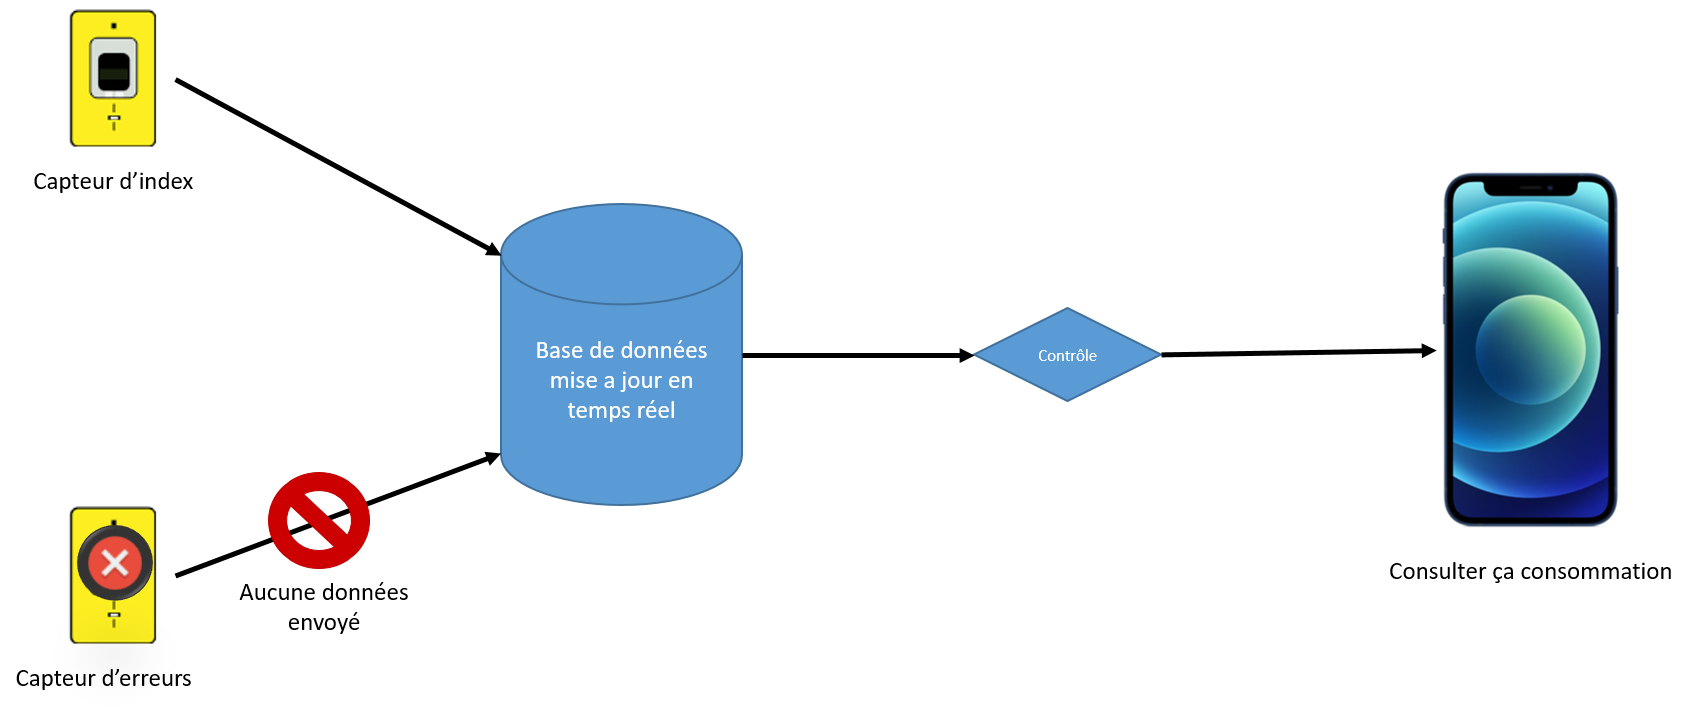
\includegraphics[scale=0.6]{img/part2/2.1.png}
	\caption{Scénario normal}
\end{figure}

\newpage

\subsection{Cas d'erreurs:}
Pour le deuxième scénario, se produit lorsqu'une erreur est détectée, le capteur d'index continue d'envoyer des données, en plus du capteur d'erreur qui intervient également en envoyant des données sur l'erreur qui s'est produite. notre système réagit différemment selon l'erreur captée:

\begin{itemize}
	\item \textbf{Surconsommation d'énergie:}

	\item \textbf{Ouverture du compteur:}

	\item \textbf{arrêt inattendu:}

	\item \textbf{Non payement:}

\end{itemize}

Le schéma suivant illustre ce cas avec les différentes erreurs:

\begin{figure}[h]
	\centering
	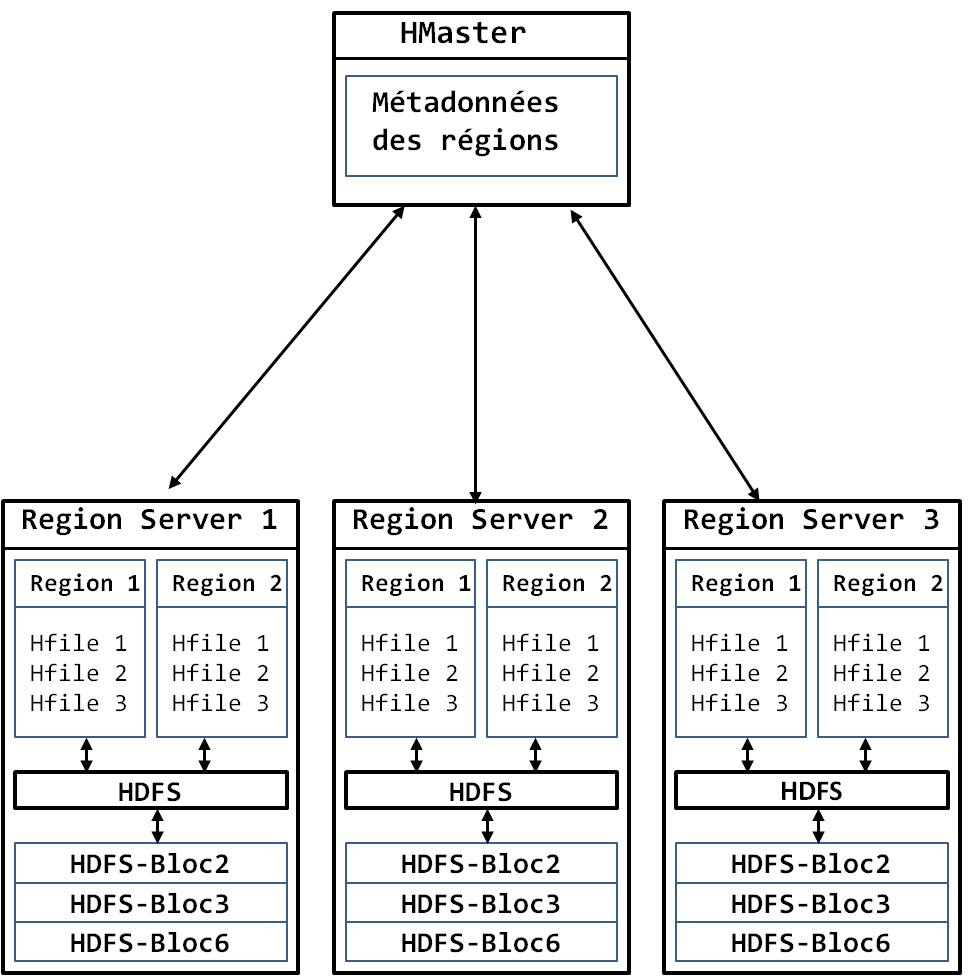
\includegraphics[scale=0.5]{img/part2/2.2.png}
	\caption{Scénario erreur}
\end{figure}
